\section*{Lab activity 1}

\subsection*{Topology diagram}
\begin{figure}[htb]
	\centering
	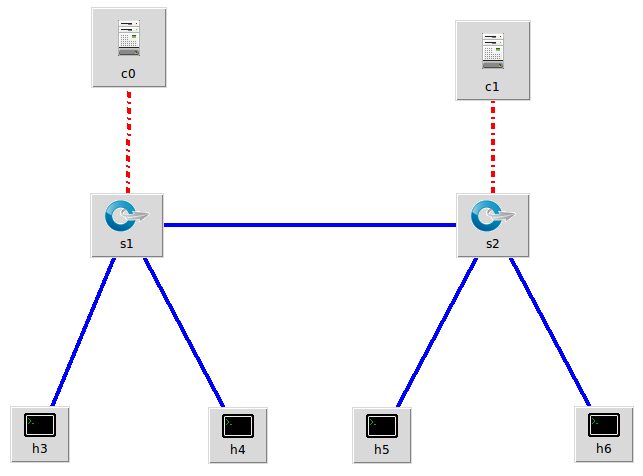
\includegraphics[width=0.8\linewidth]{img/topology-1.png}
	\caption{the topology that will be implemented during this lab activity.
  It is a simple linear topology with two switches connected to each other,
  each one connected to two hosts. Each switch is linked to a different
  SDN controller. The two controllers can be assumed local.}
	\label{fig:topology-1}
\end{figure}





\subsection*{Learning objectives}
After finishing this lab activity you will be able to:
\begin{itemize}
  \item implement a cluster of local/remote controllers inside Mininet using the Python
  middle-level Mininet API
  \item test the network connectivity of a network which
  includes a cluster of controllers and verify that its performance meets
	the requirements
  \item understand the main functions provided by the middle-level Mininet API required
  to implement a cluster of controllers
	\item understand how to set performance parameters when implementing a network
	using a Python script and the middle-level Mininet API
  \item reflect about the reasons of using more than one controller in SDN networks.
\end{itemize}






\subsection*{Scenario}
In this activity you will implement the simple topology shown in figure \ref{fig:topology-1} using
a Python script and the middle-level API provided by Mininet.
Begin by creating a new Python script, then import the Mininet classes required for
this activity and define the function that will be used to create the topology.
Inside the body of this function create a new Mininet network and add to it the
required hosts, switches, links and controllers. After writing the script, execute
it to create the network, test its connectivity and verify that the performance
meets the requirements. To conclude, answer the questions proposed in the last task.

This lab activity assumes you are proficient in SDN networks and Mininet network
emulator %(how to create a basic topology, python API, how to connect a switch to
%a remote controller,).
A basic knowledge of the Python programming language is also required.

The activity is inspired by the script \textit{controllers2.py} \cite{ref-3} included in the
examples provided by Mininet, which can therefore be used as
an additional example of how a network with multiple controllers can be implemented
inside Mininet using a Python script and the middle-level API.




\subsection*{Task 1: write the skeleton of the Python script}
\subsubsection*{Step 1}
Create a new Python script and edit it with the text editor you prefer. If you're editing
it inside the Mininet virtual machine, it is suggested to use Vim text editor.

\subsubsection*{Step 2}
Import the required Python classes from the Mininet API:
\begin{lstlisting}
#!/usr/bin/Python
from mininet.net import Mininet
from mininet.node import Controller, OVSSwitch
from mininet.cli import CLI
from mininet.log import setLogLevel, info
from mininet.link import TCLink
\end{lstlisting}

\subsubsection*{Step 3}
Define the function that will be used to create the topology:
\begin{lstlisting}
def multiControllerNet():
\end{lstlisting}

\subsubsection*{Step 4}
Inside the body of the function \code{multiControllerNet()} create a new Mininet
network:
\begin{lstlisting}
net = Mininet( controller=Controller, switch=OVSSwitch, link=TCLink )
\end{lstlisting}

The Mininet network is created invoking the Mininet constructor: the first two parameters
passed to the constructor are the classes \code{Controller} and \code{OVSSwitch}, therefore
Stanford/OpenFlow reference controllers and Open vSwitch switches will be used
in the created network. Note that these two classes are the default parameters in
the Mininet constructor, so it is not really necessary to specify them \cite{ref-4}.

The third parameter passed to the constructor is the class \code{TCLink}, which provides
performance limiting features. By using this class it is possible to set performance
parameters when creating the links of the Mininet network.

\subsubsection*{Step 6}
Make the script executable only as a program, set the CLI verbosity level to ``info''
and call the function \code{multiControllerNet()}:
\begin{lstlisting}
if __name__ == '__main__':
    setLogLevel( 'info' )
    multiControllerNet()
\end{lstlisting}
Note that the lines of code above must be placed after the function \code{multiControllerNet()}
outside its body.

\subsubsection*{Step 7}
Save the text file as ``\emph{activity-1.py}'' in your custom directory inside
the mininet virtual machine.





\subsection*{Task 2: add hosts to the network}
\subsubsection*{Step 1}
Inside the body of the function \code{multiControllerNet()} add the following line
of code in order to print to the console that hosts are being created:
\begin{lstlisting}
info( "*** Creating hosts \n" )
\end{lstlisting}

\subsubsection*{Step 2}
Still inside the body of the function \code{multiControllerNet()}, create the
four hosts required for the topology by adding them to the mininet network
previously created:
\begin{lstlisting}
h1 = net.addHost('h3')
h2 = net.addHost('h4')
h3 = net.addHost('h5')
h4 = net.addHost('h6')
\end{lstlisting}
The function used to add the hosts to the network is \code{addHost('name')}, which
accept as parameter the name of the host that will be created. The hosts names in
this network therefore will be \code{h3}, \code{h4}, \code{h5} and \code{h6}.





\subsection*{Task 3: add switches to the network}
Inside the body of the function \code{multiControllerNet()} print to the console
that switches are being created and then add to the mininet network previously
created the two switches required for the topology:
\begin{lstlisting}
info( "*** Creating switches \n" )
s1 = net.addSwitch('s1')
s2 = net.addSwitch('s2')
\end{lstlisting}







\subsection*{Task 4: create links between nodes}
Inside the body of the function \code{multiControllerNet()} print to the console
that links are being created and then add the links between the hosts and the
switches and the link between the two switches. For creating the links
use the function \code{addLink}, specifying the bandwidth and the delay for each link:
\begin{lstlisting}
info( "*** Creating links \n" )
net.addLink( h1, s1, bw=5, delay='5ms' )
net.addLink( h2, s1, bw=5, delay='5ms' )
net.addLink( h3, s2, bw=5, delay='5ms' )
net.addLink( h4, s2, bw=5, delay='5ms' )
net.addLink( s1, s2, bw=10, delay='2ms' )
\end{lstlisting}

Note that the bandwidth specified with the parameter \code{bw} is expressed in
Mbit/s, while the delay specified with the parameter \code{delay} is expressed
in milliseconds since we used the string ``ms'' (it is also possible to use
the strings ``us'' and ``s'' in order to express the delay in microseconds and
seconds) \cite{ref-7}.





\subsection*{Task 5: create the controllers}
Inside the body of the function \code{multiControllerNet()} print to the console
that reference controllers are being created and then add to the Mininet network
the two required controllers:
\begin{lstlisting}
info( "*** Creating (reference) controllers \n" )
c0 = net.addController( 'c0', port=6633 )
c1 = net.addController( 'c1', port=6634 )
\end{lstlisting}

The function used to create the controllers is \code{addController}, which accepts
as parameters the name of the controller which will be created and the TCP port that
will be used by the switches for connecting to the controller.







\subsection*{Task 6: start the mininet network}
\subsubsection*{Step 1}
Append to the body the function \code{multiControllerNet()} the following line
of code for printing to the console that the network is being started:
\begin{lstlisting}
info( "*** Starting network \n" )
\end{lstlisting}

\subsubsection*{Step 2}
Build the Mininet network:
\begin{lstlisting}
net.build()
\end{lstlisting}

\subsubsection*{Step 3}
Start the controllers:
\begin{lstlisting}
c0.start()
c1.start()
\end{lstlisting}

\subsubsection*{Step 4}
Start the switches, specifying for each switch the controller to which connect:
\begin{lstlisting}
s1.start( [ c0 ] )
s2.start( [ c1 ] )
\end{lstlisting}

\subsubsection*{Step 5}
Start the Mininet CLI:
\begin{lstlisting}
info( "*** Running CLI\n" )
CLI( net )
\end{lstlisting}

\subsubsection*{Step 6}
Stop the network so that after the user exits the Mininet CLI the network is
stopped:
\begin{lstlisting}
info( "*** Stopping network\n" )
net.stop()
\end{lstlisting}

\subsubsection*{Step 7}
Save the file and exit the text editor.

% Because each swtich has to setup one TCP connection to each controller and
% it's not possible having more than one TCP connection on the same port, so
% specifying two different ports makes it possible to connect one single switch
% to multiple controllers.



\subsection*{Task 7: execute the script and test the network}
After finishing the task 6 the script for implementing the required topology is
completed. The full script is shown in listing \ref{lst:activity-1-script} at the
bottom of this activity.

\subsubsection*{Step 1}
Execute the script as root: \\
\code{\$ sudo python activity-1.py}

\subsubsection*{Step 2}
Test the created topology: verify the network connectivity between all hosts.
Write in the lines below the commands you used and the results you obtained.

\hrulefill

\hrulefill

\hrulefill

\hrulefill

\subsection*{Step 3}
Verify that the bandwidth and the delay of each link comply with the values
specified in the topology diagram shown in figure \ref{fig:topology-1}.
Write in the lines below the commands you used and the results you obtained.

\hrulefill

\hrulefill

\hrulefill

\hrulefill




\subsection*{Task 8: reflection}
\subsubsection*{1 - What are the advantages of having more controllers instead of one
single controller which serves all the switches of the network?}
\hrulefill

\hrulefill

\hrulefill

\hrulefill

\subsubsection*{2 - Would the fault tolerance of the network shown in figure \ref{fig:topology-1}
change if only one controller (linked to both the switches) was used
instead of two?}
\hrulefill

\hrulefill

\hrulefill

\hrulefill



\subsubsection*{3 - In this activity the topology shown in figure \ref{fig:topology-1}
was implemented assuming that the two controllers were local controllers. How would
you have to change the Python script you created in this activity in order
to use remote controllers instead of local ones? (Hint: see reference \cite{ref-5})}
\hrulefill

\hrulefill

\hrulefill

\hrulefill



\subsubsection*{4 - How could we improve the fault tolerance of the netowork shown
in figure \ref{fig:topology-1} making minor changes to the Python script used?}
% Each switch connected to both controllers, each controller
% could be a distributed controller
\hrulefill

\hrulefill

\hrulefill

\hrulefill



\lstset{
 upquote=true,
 showspaces=false,
 showtabs=false,
 frame=single,
 tabsize=2,
 breaklines=true,
 numbers=left,
 showstringspaces=false,
 breakatwhitespace=true,
 escapeinside={(*@}{@*)},
 keywordstyle=\bfseries,
 basicstyle=\scriptsize\ttfamily,
}

\begin{minipage}{\linewidth}
\begin{lstlisting}[label=lst:activity-1-script, caption=the complete Python script required for Activity 1]
#!/usr/bin/Python
from mininet.net import Mininet
from mininet.node import Controller, OVSSwitch
from mininet.cli import CLI
from mininet.log import setLogLevel, info
from mininet.link import TCLink

def multiControllerNet():
    net = Mininet( controller=Controller, switch=OVSSwitch, link=TCLink )

    info( "*** Creating hosts\n" )
    h1 = net.addHost('h3')
    h2 = net.addHost('h4')
    h3 = net.addHost('h5')
    h4 = net.addHost('h6')

    info( "*** Creating switches\n" )
    s1 = net.addSwitch( 's1' )
    s2 = net.addSwitch( 's2' )

    info( "*** Creating links\n" )
    net.addLink( h1, s1, bw=5, delay='5ms' )
    net.addLink( h2, s1, bw=5, delay='5ms' )
    net.addLink( h3, s2, bw=5, delay='5ms' )
    net.addLink( h4, s2, bw=5, delay='5ms' )
    net.addLink( s1, s2, bw=10, delay='2ms' )

    info( "*** Creating (reference) controllers\n" )
    c0 = net.addController( 'c0', port=6633 )
    c1 = net.addController( 'c1', port=6634 )

    info( "*** Starting network\n" )
    net.build()
    c0.start()
    c1.start()
    s1.start( [ c0 ] )
    s2.start( [ c1 ] )

    info( "*** Running CLI\n" )
    CLI( net )

    info( "*** Stopping network\n" )
    net.stop()

if __name__ == '__main__':
    setLogLevel( 'info' )
    multiControllerNet()
\end{lstlisting}
\end{minipage}
